\part{Proposition de corrigé et beaucoup plus long encore pour ce titre}

\vspace{0.9em}

\section{Rappel du sujet~:~\textit{Transformation} de Laplace et beaucoup plus long encore pour ce titre}

\begin{citation}
    dfdf \\
    sdsd
\end{citation}

\subsection{Test d'un module "\textit{bloc encadré}" et beaucoup plus long encore pour ce titre de sous-section}

\begin{boxFill}
\pictoBook{} \uLine[secondary]{\textbf{\Large Pour en savoir plus}}

\vspace{0.5em}

\begin{uList}[diamond][secondary]
\item JOUANNEAU D., « Un arc de crise sous-estimé : Inde-Pakistan-Afghanistan », \textit{Revue Défense Nationale}, n°831, juin 2020, p. 137-146
\item S. LANDRIN, G. DELACROIX, \textit{Dans la tête de Narendra Modi}, Paris, Solin/Actes Sud, 2024
\item D. LAPIERRE, L. COLLINS, \textit{Cette nuit la liberté}, 1975, nombreuses éditions en poche. Récit par deux journalistes des débats qui ont mené à l'indépendance de l'Inde. Se lit comme un roman.
\item Analyse sur France 24 par un spécialiste : \url{https://www.france24.com/fr/vidéo/20250511-escalade-entre-l-inde-et-le-pakistan-analyse-de-jean-luc-racine}
\item Historique rapide des tensions : \url{https://www.youtube.com/watch?v=arGoUba-bC8}
\item Cérémonie spectaculaire de fermeture de la frontière entre les deux pays : \url{https://www.dailymotion.com/video/x3kokkn}
\end{uList}
\end{boxFill}

Lorem ipsum dolor sit amet, consectetur adipiscing elit. Soit \( f : \mathbb{R} \to \mathbb{R} \) une fonction différentiable telle que \( f'(x) = \sin(x) \). Intégrons cette fonction sur l'intervalle \([a,b]\) :

\[
\int_a^b f'(x) \, dx = f(b) - f(a).
\]

Sed do eiusmod tempor incididunt ut labore et dolore magna aliqua. Considérons la série de Fourier de la fonction \(g\) définie par

\[
g(x) = \sum_{n=1}^\infty a_n \cos(nx) + b_n \sin(nx),
\]

où les coefficients \(a_n\) et \(b_n\) satisfont les conditions de convergence. 

Ut enim ad minim veniam, quis nostrud exercitation ullamco laboris nisi ut aliquip ex ea commodo consequat. L'équation aux dérivées partielles

\[
\frac{\partial u}{\partial t} = \alpha \frac{\partial^2 u}{\partial x^2}
\]

modélise la diffusion thermique dans une barre homogène, où \(\alpha\) est le coefficient de diffusion thermique. 

Duis aute irure dolor in reprehenderit in voluptate velit esse cillum dolore eu fugiat nulla pariatur. Pour tout espace vectoriel \(V\) de dimension finie, le théorème de dimension stipule que

\[
\dim(V) = \dim(\ker T) + \dim(\mathrm{im} \, T),
\]

pour tout opérateur linéaire \(T : V \to W\).

\subsection{Abscisse de convergence}


Lorem ipsum dolor sit amet, consectetur adipiscing elit. Soit \( f : \mathbb{R} \to \mathbb{R} \) une fonction différentiable telle que \( f'(x) = \sin(x) \). Intégrons cette fonction sur l'intervalle \([a,b]\) :

\[
\int_a^b f'(x) \, dx = f(b) - f(a).
\]

Sed do eiusmod tempor incididunt ut labore et dolore magna aliqua. Considérons la série de Fourier de la fonction \(g\) définie par

\[
g(x) = \sum_{n=1}^\infty a_n \cos(nx) + b_n \sin(nx),
\]

où les coefficients \(a_n\) et \(b_n\) satisfont les conditions de convergence. 

Ut enim ad minim veniam, quis nostrud exercitation ullamco laboris nisi ut aliquip ex ea commodo consequat. L'équation aux dérivées partielles

\[
\frac{\partial u}{\partial t} = \alpha \frac{\partial^2 u}{\partial x^2}
\]

modélise la diffusion thermique dans une barre homogène, où \(\alpha\) est le coefficient de diffusion thermique. 

Duis aute irure dolor in reprehenderit in voluptate velit esse cillum dolore eu fugiat nulla pariatur. Pour tout espace vectoriel \(V\) de dimension finie, le théorème de dimension stipule que

\[
\dim(V) = \dim(\ker T) + \dim(\mathrm{im} \, T),
\]

pour tout opérateur linéaire \(T : V \to W\).

\subsection{Quelques propriétés de la transformée de Laplace}


Lorem ipsum dolor sit amet, consectetur adipiscing elit. Soit \( f : \mathbb{R} \to \mathbb{R} \) une fonction différentiable telle que \( f'(x) = \sin(x) \). Intégrons cette fonction sur l'intervalle \([a,b]\) :

\[
\int_a^b f'(x) \, dx = f(b) - f(a).
\]

Sed do eiusmod tempor incididunt ut labore et dolore magna aliqua. Considérons la série de Fourier de la fonction \(g\) définie par

\[
g(x) = \sum_{n=1}^\infty a_n \cos(nx) + b_n \sin(nx),
\]

où les coefficients \(a_n\) et \(b_n\) satisfont les conditions de convergence. 

Ut enim ad minim veniam, quis nostrud exercitation ullamco laboris nisi ut aliquip ex ea commodo consequat. L'équation aux dérivées partielles

\[
\frac{\partial u}{\partial t} = \alpha \frac{\partial^2 u}{\partial x^2}
\]

modélise la diffusion thermique dans une barre homogène, où \(\alpha\) est le coefficient de diffusion thermique. 

Duis aute irure dolor in reprehenderit in voluptate velit esse cillum dolore eu fugiat nulla pariatur. Pour tout espace vectoriel \(V\) de dimension finie, le théorème de dimension stipule que

\[
\dim(V) = \dim(\ker T) + \dim(\mathrm{im} \, T),
\]

pour tout opérateur linéaire \(T : V \to W\).
\begin{boxFill}[primary] 
Ce texte représente un texte que l'on peut mettre dans un encadré 1\footnote{Ceci est une note, séparée du texte principal par un petit trait coloré.}.
\end{boxFill}


\begin{boxBorder}[secondary]
Ce texte représente un texte que l'on peut mettre dans un encadré 3
\end{boxBorder}

\cartouche[primary]{Question au programme}

venisin ihicil ide non placcus essi \textit{optaerro} odiorro magnim nis dis et, ipitaesto tem velit, sa sita sa nobis dolore quod quia dolorro \textbf{\textit{eostecabor}} andit, etus cum et est eumquia \textbf{facescipsant} et eos moluptatur\footnote{Ceci est une note, séparée du texte principal par un petit trait coloré.} audit volut utem ratinveribus magnimo lectur?

\vspace{0.5em}

\cartouche[secondary]{Question au programme}

Lorem Ipsum

\begin{boxCard}[primary]{Question au programme}
Ceci est le texte de mon encadré.
Il est dans une boîte rectangulaire avec fond.
\end{boxCard}



\part{Proposition de corrigé}

\vspace{1em}

{\arrayrulecolor{secondarycolor}
\begin{tabular}{| T{0.13\linewidth} |T{0.13\linewidth} | T{0.13\linewidth}|}
\multicolumn{1}{p{0.13\linewidth}}{\cartoucheun{Algèbre}} &
\multicolumn{1}{p{0.13\linewidth}}{\cartoucheun{Analyse}} &
\multicolumn{1}{p{0.13\linewidth}}{\cartoucheun{Probabilités}} \\
il était & est & bouh \\
\hline
était & tt & bouh \\
\hline
\multicolumn{3}{|c|}{\cellcolor{background1}\textbf{Ligne fusionnée sur trois colonnes}} \\
\hline
était & tt & bouh \\
\hline
\end{tabular}}

\begin{center}
{\arrayrulecolor{primarycolor}
\begin{tabular}{|T{0.13\linewidth} |T{0.55\linewidth}| }
\multicolumn{1}{p{0.13\linewidth}}{\cartouchedeux{Année et plus encore !}} &
\multicolumn{1}{p{0.55\linewidth}}{\cartouchedeux{Evénements}} \\
  1903 & Premier événement \\
  \hline
  1911 & deuxième événement particulièrement tragique\\
  \hline
  \multicolumn{2}{|c|}{\cellcolor{background2}\textbf{Ligne fusionnée sur deux colonnes}} \\
  \hline
  1913 & le troisième\\
  \hline
  1922 & le soleil brille  \\
  \hline
\end{tabular}}
\end{center}

\section{Quelques modules}


\pictoExergue[secondary] Texte normal

\pictoExergue[primary] Texte normal
\normalsize

\pictoExergue[secondary][8mm] test
\pictoExergue[secondary][16mm] test

\subsection{Les listes à puces}

\begin{uList}[dash][secondary]
  \item Test
\end{uList}

\begin{uList}[diamond][primary]
  \item Losange primaire.
\end{uList}
\begin{uList}[bullet][secondary]
  \item Test
\end{uList}


\begin{uList}[diamond][secondary]
  \item Losange primaire.
\end{uList}

\begin{uList}[bullet][primary]
  \item Texte normal
\end{uList}

{\Large
\begin{uList}[bullet][primary]
  \item Texte large
\end{uList}
}

{\tiny
\begin{uList}[diamond][secondary]
  \item Texte minuscule
\end{uList}
}

\subsection{Les listes numérotées}
\begin{oList}[arabic][secondary]
  \item Premier
  \item Deuxième
\end{oList}

\begin{oList}[alph][secondary]
  \item Premier
  \item Deuxième
\end{oList}

\begin{oList}[Roman][primary]
  \item Premier
  \item Deuxième
\end{oList}

\subsection*{Citations}

\begin{citation}[primary]
« Les mathématiques possèdent non seulement la vérité,
mais une beauté suprême. »
\end{citation}

\begin{citation}[secondary]
Attention : dans ce problème, les questions sont indépendantes et ne sont pas classées par difficulté.
\end{citation}

\subsection*{Highlights}
\par

{\LARGE \triple{primary}{\robotoCondensed\bfseries {Résultat fondamental}}}

\chevron{secondary}{\robotoCondensed\bfseries Résultat fondamental}


\normalfont 

\uLine[secondary]{Texte souligné en secondarycolor}



\textbf{Note au candidat :}


\begin{sideLine}{primary}
Texte important.
\end{sideLine}

\begin{sideLine}{secondary}
Texte secondaire.
\end{sideLine}


\subsection*{Notes de pied de pages}


Voici un texte avec une note de bas de page \footnote{Ceci est une note, séparée du texte principal par un petit trait coloré.}
Un autre exemple avec plusieurs notes\footnote{Une deuxième note.}\footnote{Et une troisième pour montrer la continuité.}


\subsubsection{Test}

modélise la diffusion thermique dans une barre homogène, où \(\alpha\) est le coefficient de diffusion thermique.

Duis aute irure dolor in reprehenderit in voluptate velit esse cillum dolore eu fugiat nulla pariatur. Pour tout espace vectoriel \(V\) de dimension finie, le théorème de dimension stipule que

\subsubsection{Test}

Duis aute irure dolor in reprehenderit in voluptate velit esse cillum dolore eu fugiat nulla pariatur. Pour tout espace vectoriel \(V\) de dimension finie, le théorème de dimension stipule que

\subsubsection{Test et exceptionnellement plus long encore pour ce titre de sous-sous-section pourtant peu utilisé dans ces proprotions}

Duis aute irure dolor in reprehenderit in voluptate velit esse cillum dolore eu fugiat nulla pariatur. Pour tout espace vectoriel \(V\) de dimension finie, le théorème de dimension stipule que

\begin{boxBorder}[secondary]
\pictoBook{}
\uLine[primary]{Entrainez-vous}
\end{boxBorder}


\subsection{Notes de \TitleTextIt{pied de pages}}


\subsection*{Notes de pied de pages}
\subsection*{Notes de pied de pages}
\subsection*{Notes de pied de pages}


\begin{figure}[h]
    \centering
    % Le texte alternatif est maintenant géré nativement via la clé "alt"
    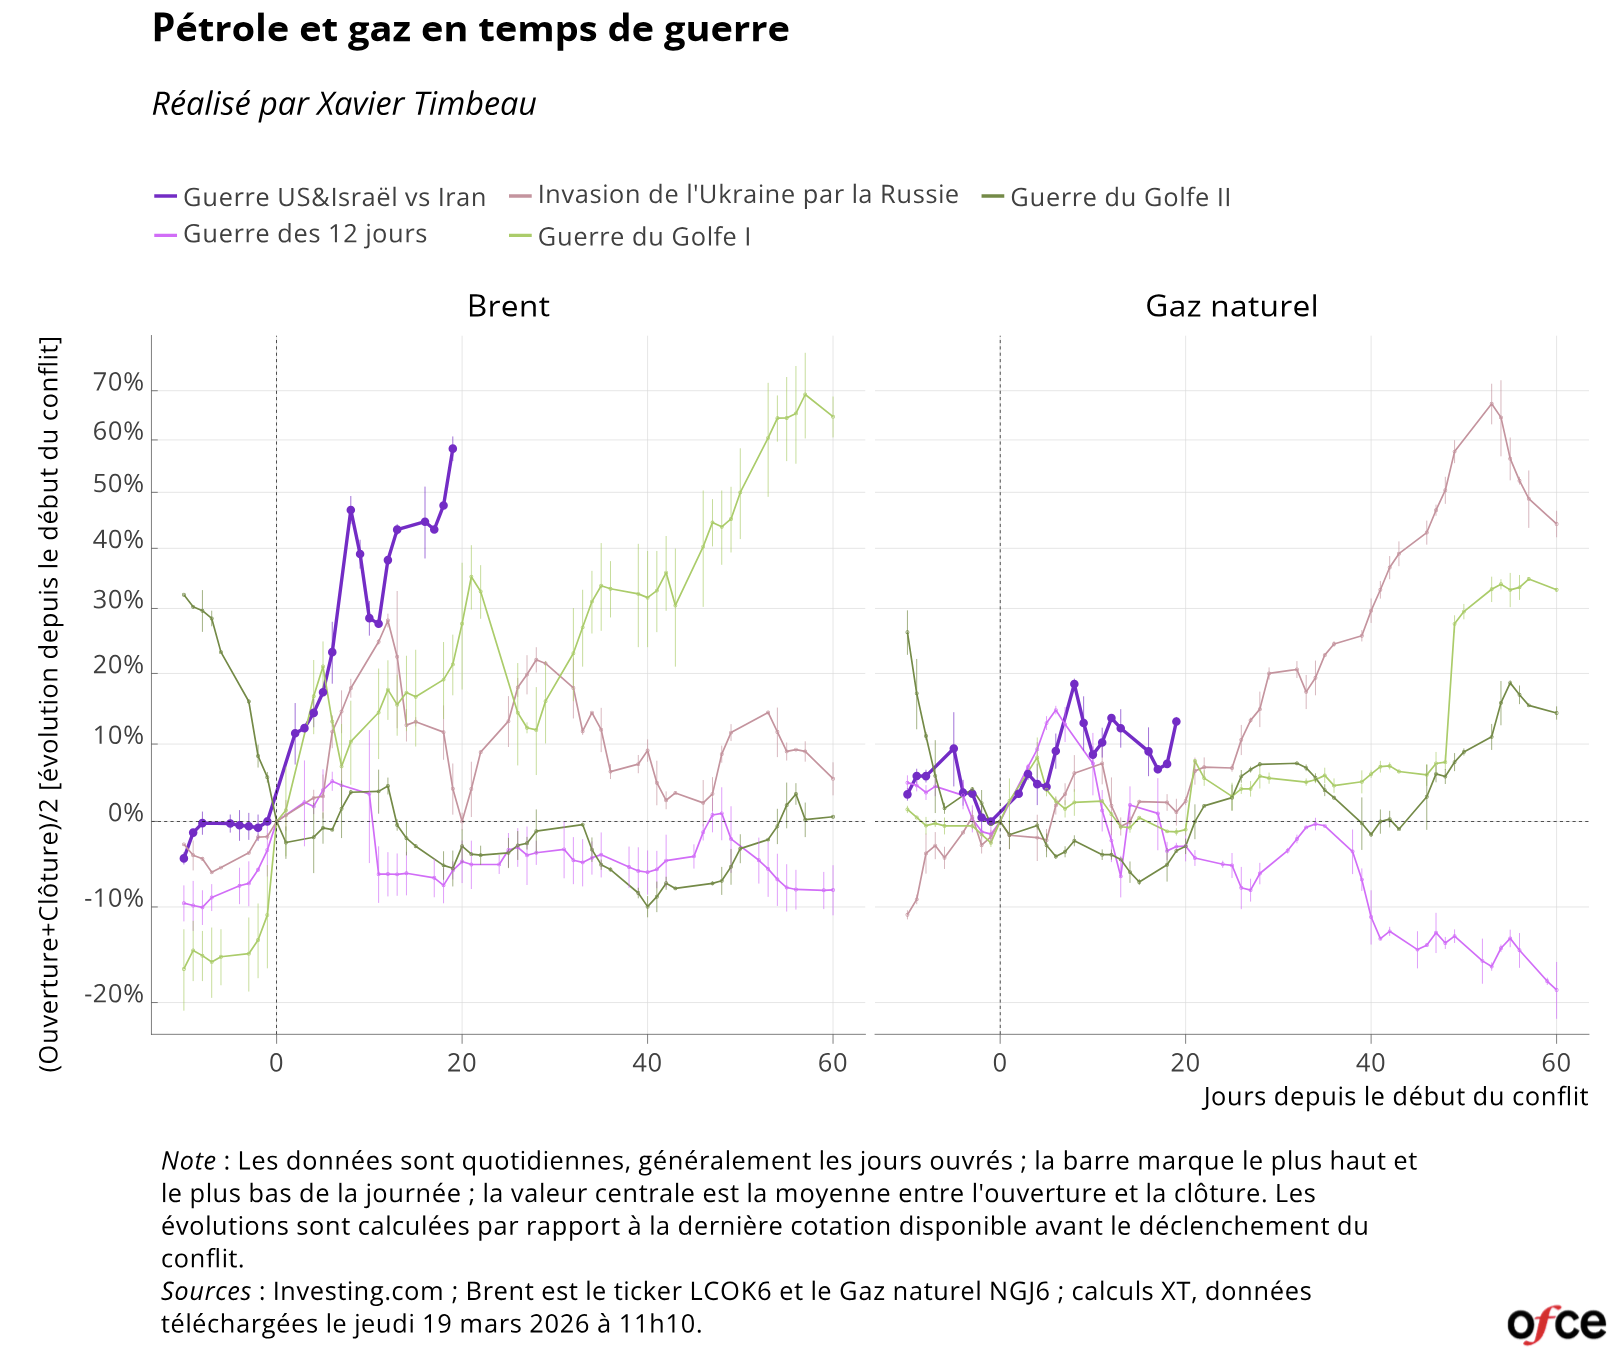
\includegraphics[width=\textwidth, alt={Graphique comparant l'évolution quotidienne du prix du pétrole (Brent) et du gaz naturel (GNL) lors de cinq conflits récents au Moyen-Orient. La courbe du conflit Iran 2026 se distingue par une hausse du Brent de 40 à 60\% en moins de 20 jours, surpassant en vitesse et en amplitude les épisodes précédents. L'impact sur le gaz reste plus modéré, inférieur à +30\% sur la même période.}]{img/image-graphique.png}
    \caption{\textbf{Comparaison de l'évolution des prix du pétrole (Brent) et du gaz naturel lors de cinq conflits récents au Moyen-Orient (base\,100 = dernier cours avant le déclenchement de chaque conflit)}}
\sourceimage{Graphique de l'évolution des prix du pétrole et du gaz}{\href{https://www.ofce.sciences-po.fr/blog2024/fr/2026/20260310_XT_gow/}{OFCE}, mars 2026}
\end{figure}


\part{Test}

\pictoCheck \pictoBook \pictoChrono  
\pictoGoal \pictoLink \pictoMedia
\pictoMemo \pictoNote \pictoQuestion
\pictoRec \pictoTime \pictoWarning
\pictoZoom 

\hspace{5em}

\pictoCompEcrite
\pictoCompOrale
\pictoFar \pictoGear \pictoOnlineActivity \pictoOrientation 
\pictoPrerequis \pictoProdOrale \pictoOraleContinue 
\pictoOraleInteraction \pictoSolution \pictoSupportAudio \pictoSupportVideo \pictoSurligner \pictoSynthese \pictoTempsEstime

\pictoTips

\pictoExergue






\paragraph{Test sans majuscule}

\url{www.test.com}
\url{https://www.youtube.com/watch?v=arGoUba-bC8}

\subsection*{Notes de pied de pages}
\subsection*{Notes de pied de pages}
\subsection*{Notes de pied de pages}
\subsection*{Notes de pied de pages}
\subsection*{Notes de pied de pages}
\subsection*{Notes de pied de pages}
\subsection*{Notes de pied de pages}
\subsection*{Notes de pied de pages}
\subsection*{Notes de pied de pages}

\subsection*{Notes de pied de pages}
\subsection*{Notes de pied de pages}
\subsection*{Notes de pied de pages}

% =================================================================
% Théorème : Règle de la chaîne généralisée
% =================================================================


    
%%%
%\end{theorem}

% =================================================================
% Packages nécessaires à inclure dans le préambule :
% =================================================================
% \usepackage{amsmath}     % Pour les environnements mathématiques avancés
% \usepackage{amssymb}     % Pour les symboles mathématiques (\mathbb, etc.)
% \usepackage{amsthm}      % Pour l'environnement theorem
% 
% Définition de l'environnement theorem (à placer dans le préambule) :
% \newtheorem{theorem}{Théorème}[section]
% Cette ligne crée un environnement "theorem" qui affichera "Théorème" 
% suivi d'un numéro qui se remet à zéro à chaque section